\chapterauthor{Strategy \& Stakeholder Analysis}{Paul Vogelberg}
\contribution{Paul Vogelberg}

\section{Introduction to the Strategic Pivot}

The UK Connected and Automated Mobility (CAM) sector faces a critical simulation-to-reality gap; regulators and insurers demand exhaustive physical edge-case validation before approving autonomous deployments, yet Original Equipment Manufacturers (OEMs) lack the agile hardware to safely execute these collisions. To address this bottleneck, our enterprise executes a foundational strategic manoeuvre: pivoting from the development and sale of a physical engineering asset (the AEB Rabbit) to providing a comprehensive Testing-as-a-Service (TaaS) platform. This allows autonomous vehicle (AV) developers to access high-fidelity, physical validation data without bearing the cost of maintaining their own target fleets.

This service model is enabled by our vehicle's specialised engineering architecture. Designed for rapid acceleration rather than cruising, the AEB Rabbit utilises a supercapacitor energy storage system to execute repeatable,  les than 10-second "panic" manoeuvres that mimic erratic human behaviour. To guarantee the high track utilisation required for TaaS profitability, the platform employs a modular supply chain strategy. By standardising replaceable impact shells and maintaining a buffer of drivetrain components, the enterprise ensures swift track-side mechanical recovery following a severe collision, protecting operational throughput.

Strategically, our Go-To-Market plan bypasses individual OEM bureaucratic delays by natively integrating the AEB Rabbit directly into established CAM Testbed UK facilities. Here, the enterprise serves as an ethical and legal buffer for AV developers. By operating strictly within defined Operational Design Domains (PAS 1883), governed by Safety Management Systems (PAS 1881), and providing immutable "black box" telemetry (PAS 1882), we absorb the physical risks of extreme edge-case testing. This provides the undeniable empirical evidence required by insurers and regulators to safely determine liability in a post-human-driver landscape.

Finally, this enterprise achieves rigorous environmental alignment without compromising commercial viability. At the macro level, the TaaS model operates as a Use/Result-Oriented Product-Service System (PSS), aggregating industry demand and preventing redundant OEM hardware manufacturing. Because the enterprise retains asset ownership under this model, we are financially incentivised to execute the 9R Circular Economy Framework. Sustainability is actively achieved through inherited lifecycle extension: utilising high-duty cycle supercapacitors, instituting drivetrain remanufacturing loops, and deploying recyclable Expanded Polypropylene (EPP) sacrificial shells to drastically reduce the operation's embodied carbon.

\section{Macro-Environmental Dynamics and the UK Ecosystem}

Our strategy leverages the government's investment focus, as outlined in the Zenzic UK CAM Roadmap, and capitalises on established CAM Testbed facilities.

\subsection{The Zenzic UK CAM Roadmap}

The most critical macro-environmental tool available for this analysis is the UK Connected and Automated Mobility (CAM) Roadmap to 2035, coordinated by Zenzic, a joint venture between UK industry and government \cite{zenzic_about}. The Roadmap acts as a comprehensive vision of the path required to create scalable solutions and bring CAM technologies to reality.

According to the executive summary \cite[p.~5,11,14]{cracknell_2023}, despite aggressive timelines to deploy self-driving vehicles by 2025, the UK AV sector is currently bottlenecked by a lack of physical, real-world validation. Regulators are hesitant to approve deployments without overwhelming proof of safety, and OEMs are concerned that a single public incident will derail their progress. The industry cannot scale until it can rigorously and safely physically test edge-cases.

Our testing vehicles provide the critical, physical validation layer required to bridge the gap between simulation and public deployment. We allow our clients to safely generate the hard data needed to satisfy regulators, achieve pre-certification, and protect their brand reputation from public accidents.

The total addressable market is expanding rapidly due to acute global labour shortages in freight, logistics, and public transport \cite[p.~6]{wef_2021}. Because operators are forced to adopt No-User-in-Charge (NUiC) vehicles to survive, OEMs are scaling their platforms faster than ever to meet this structural deficit \cite[p.~9,11,17]{cracknell_2023}. Every new platform and iteration requires exhaustive physical testing, creating a recurring, high-volume demand for our validation equipment.  
This venture is strategically aligned with the Centre for Connected and Autonomous Vehicles' (CCAV) ongoing Automated Vehicles Act implementation programme \cite{lawcom_avs_2024}, which fundamentally transitions the UK from regulatory theory into active commercial deployment % [Paul Vogelberg: Source also for this?]
. Concurrently, the Zenzic roadmap identifies the rapid acceleration of the domestic CAM supply chain as a primary macro-environmental driver for the sector \cite[p.~9,10,19]{cracknell_2023}. As the government actively seeks to build a world-class, sovereign CAM ecosystem with a strict legislative emphasis on physical safety assurance, our enterprise is ideally positioned to capture targeted grant funding. By aligning our business with the criteria of active government initiatives, specifically the £150 million CAM Pathfinder Programme to accelerate commercial market readiness \cite{pockney_2026}, we can leverage state-sponsored funding to integrate our physical validation tools directly into the UK's deployment infrastructure.

\subsection{Utilising CAM Testbed UK}

The UK offers a highly concentrated target market through 'CAM Testbed UK', a unified network of world-leading physical and virtual testbeds. Because safety-critical edge cases occur rarely and are dangerous to replicate in real-world traffic, developers cannot rely on waiting for them to naturally occur on public roads \cite[p.~12]{chen_2024}. Our vehicles solve this by allowing test engineers to repeatedly and safely recreate high-stakes, erratic scenarios in controlled environments. This rigorous scenario-based testing directly assists OEMs in meeting the BSI PAS 1881 standard to reduce testing risks to a level that is as low as reasonably practicable (ALARP) \cite[p.~1]{pas1881}, thereby fortifying their Operational Safety Case for regulatory approval.

Our system acts as the essential physical ground-truth required to validate the UK's investments in virtual simulation. Our product enables state-of-the-art facilities to correlate their virtual 'digital-twin' testing with real-world sensor data. Instead of focusing on targeting individual OEMs, with a heavy customer acquisition cost and prolonged procurement cycle, our strategy natively integrates the platform into the service offerings of centralised CAM Testbed facilities. This positioning establishes the enterprise as an indispensable, embedded supplier to the global testing hubs where the entire autonomous mobility industry already meets.

There is an established, proven precedent of demand within the CAM Testbed UK network for our precise technology. For instance, during the recent £5.8M project at the Culham Science Centre (a CAM Testbed UK facility), the delivery partners explicitly utilised government grant funding to purchase a motorised pedestrian dummy to increase their safety testing options \cite[p.~2]{culham_2024}. While these testbeds are currently investing in low-speed pedestrian targets, our TaaS model builds upon this precedent by filling the unaddressed, high-value gap for highly dynamic, high-mass vehicular targets. Our business is perfectly timed to capture this active, ongoing capital expenditure from UK testing facilities looking to maintain their global competitiveness % [Paul Vogelberg: Could explain how our service builds on this precedent. Maybe not precisely our service, need to clarify what our dummy represents in testing scenarios.]
.

\section{Manoeuvring to the Testing-as-a-Service (TaaS) Model}

As autonomous vehicle (AV) architectures evolve from modular pipelines to end-to-end (E2E) AI systems, an emerging market demand has surfaced for advanced dynamic testing. E2E systems frequently suffer from "causal confusion"—a critical failure mode where the model relies on spurious, false correlations that ultimately lead to catastrophic failures during real-world deployment \cite[p.~11-2]{chen_2024}. While developers primarily evaluate these models through offline, open-loop frameworks, the literature explicitly warns that such methods fail to measure a system's ability to recover from physical drift and do not provide conclusive evidence of safe driving behaviour \cite[p.~7]{chen_2024}. Consequently, rigorous, closed-loop dynamic benchmarking is not just beneficial, but fundamentally required.

Rather than relying on the traditional automotive diagnostic model that forces end-users into capital-intensive (CAPEX) hardware purchases, our enterprise addresses this critical evaluation gap through a TaaS delivery model. By strategically pivoting our physical engineering asset to a service-based approach, we equip client organisations, such as EV start-ups and OEM innovation divisions, % [Paul Vogelberg: insert reference to Toby's work]
with the dynamic, closed-loop physical environments required to expose and resolve causal confusion cost-effectively. Crucially, this model absorbs the operational burdens of hardware maintenance, infrastructure, and rapid technological obsolescence.

\subsection{Hardware Specialisation: The "Sprint" Advantage}

This TaaS strategy is explicitly necessitated by the unique mechanical profile of our adapted Formula Student (FS) architecture. The AEB Rabbit is not designed for a long duty cycle, but for short highly explosive acceleration, possessing a maximum power output lifetime of approximately 6 seconds per duty cycle % [Paul Vogelberg: source to engineering report figures here]
.

While this short operational runtime could render the vehicle unviable as a traditional commercial product for direct purchase, it is the performance envelope required to simulate extreme, dynamic edge cases (such as an erratic pedestrian darting into traffic, or a fast vehicle cutting across lanes). In our model, the client purchases the accurate data generated from a "panic" manoeuvre. Behind the scenes, our enterprise manages the operational duty cycle, using our accumulator system capability of rapid charging, reliable thermal management and consistent runs due to its supercapacitor architecture % [Paul Vogelberg: source to engineering report figures here]
, providing seamless and reliable value to the client.

\subsection{Full-Service Integration over Hardware Rental}

Our TaaS model fundamentally lowers this barrier to entry. By providing the self-propelled target, the trained safety operators, compliant with PAS 1884 \cite{pas1884}, and the continuous data-logging architecture, compliant with PAS 1882 \cite{pas1882}, we eliminate the need for our clients to train their own staff on complex, hazardous testing procedures. The client can simply dictate the conditions in which their automated vehicle should safely operate, the Operational Design Domain (ODD) parameters, and our enterprise can execute the required scenario to deliver the empirical data required for their safety cases.

\subsection{Supply Chain and Margin Defensibility}

The commercial viability of this TaaS model relies heavily on high utilisation rates and minimal track downtime. Because the AEB Rabbit will inevitably be subjected to physical impacts during edge-case validation, traditional testing rigs could suffer catastrophic, costly downtime.

Our platform utilises a modular architectural design, which ensures sustained profitability. By using standardised components and classifying them based on wear and collision-probability, our supply chain strategy can enable rapid, track-side mechanical recovery for the most likely repairs. This modularity prevents the total loss of the asset during a collision and isolates damage to affordable, replaceable outer components while protecting the high-value drivetrain. This strategic resilience secures consistent test throughput, directly underpinning the enterprise's robust operational expenditure (OPEX) forecasts and ensuring a predictable return on investment (ROI).

\section{Stakeholder Salience Identification}

\subsection{Introduction to the model}

\begin{figure}[h]
\centering
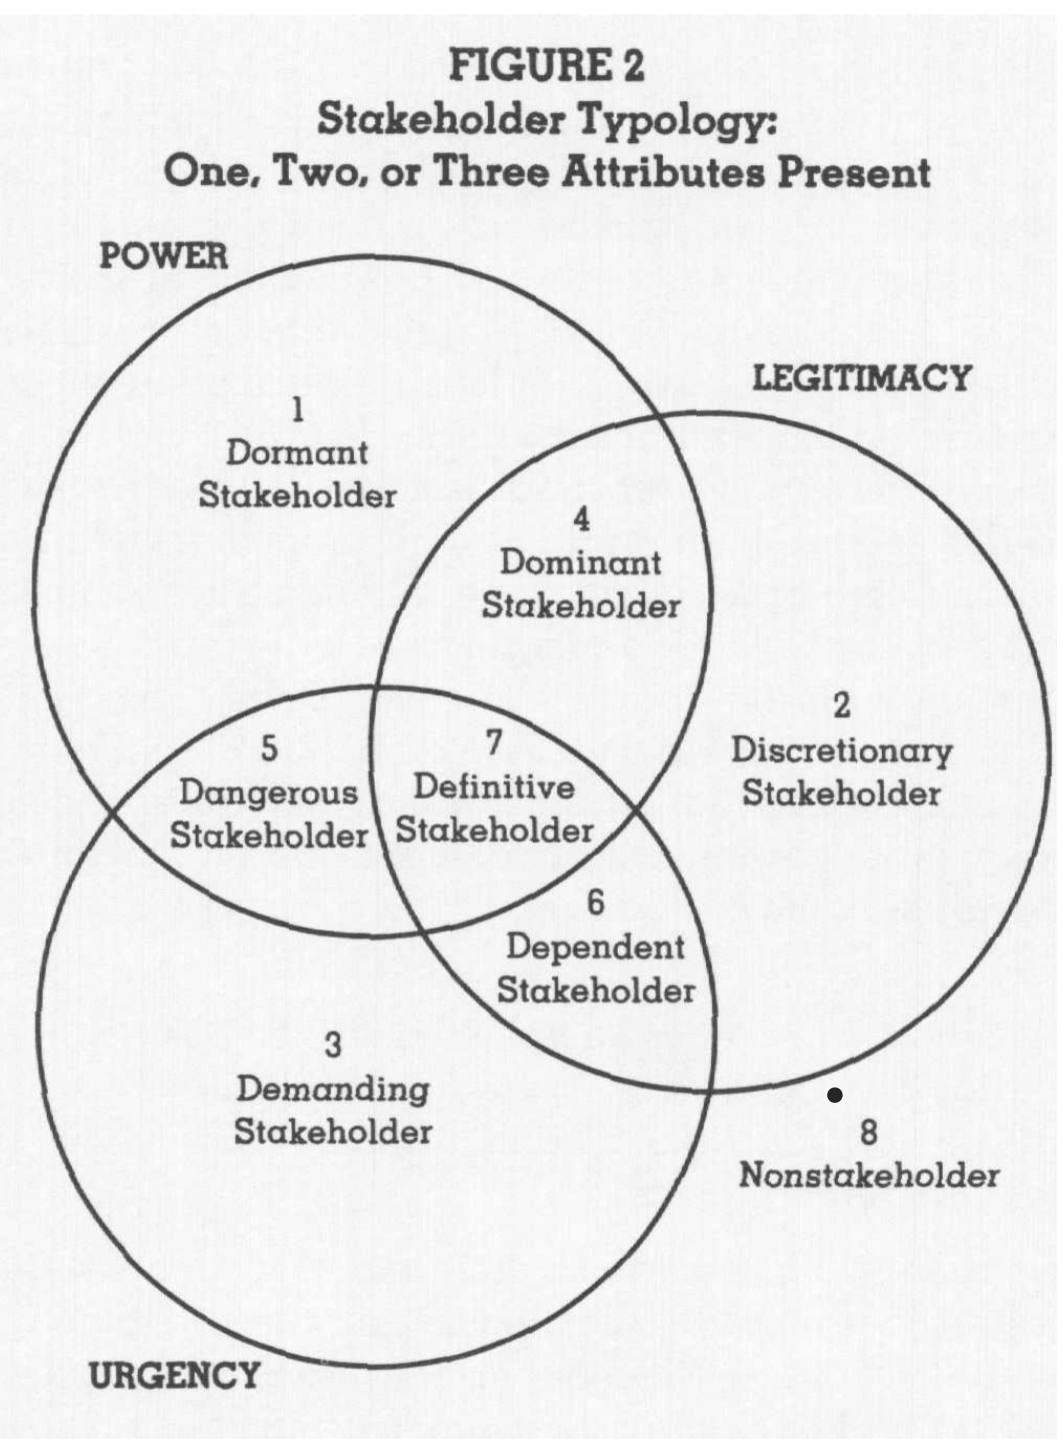
\includegraphics[width=0.6\textwidth]{figures/Figure1.jpeg}
\caption{Stakeholder Typology}
\end{figure}


While traditional matrices (such as RACI) map static operational responsibilities, the high-risk, heavily regulated nature of the CAM sector demands a dynamic framework for strategic resource allocation. The Mitchell et al. Stakeholder Salience Model \cite{mitchell_1997} is explicitly appropriate for this enterprise because it accounts for rapid, event-driven shifts in stakeholder priority and allows the management team to focus its limited engagement capital toward actors possessing two or more salience attributes. The model uses the triad: Power, Legitimacy, Urgency, for which a stakeholder can be assigned to a certain category using Figure 1.

In accordance with Proposition 1a, which asserts that 'stakeholder salience will be low where only one of the stakeholder attributes (power, legitimacy, and urgency) is perceived by managers to be present' \cite[p.~874]{mitchell_1997}, this report focuses its active engagement strategy on stakeholders possessing two or more of these attributes.

For every such class, the applicable stakeholders are given and the reasoning is explained:

\begin{itemize}
  \item Definitive Stakeholders - Insurers \& Testbed Operators: these actors possess all three attributes. Insurers hold financial power and legal legitimacy over operations, while their need for immediate post-incident data drives high urgency. Similarly, testbed operators have the power and legitimacy to halt trials instantly to protect their track's safety. Whilst the possibility of utilising OEMs' testing facilities exists, our market analyse shows that we should focus on EV start-ups and OEM innovation divisions.
  \item Dominant Stakeholders - Regulators \& Highway Authorities: entities such as CCAV hold ultimate regulatory power and legitimacy but generally exhibit lower urgency during day-to-day closed-track testing % [Paul Vogelberg: find source]
, as under Mitchell's theory, their urgency is typically event-driven and only spikes post-incident, provided compliance is maintained.
  \item Dependent Stakeholders - General Public: this group hold high moral legitimacy and urgency regarding their physical safety, but lack the direct power to enforce testing protocols, relying instead on our internal ethics governance.
  \item Dangerous Stakeholders - Cyber-Threat Actors: whilst this actor does not possess any legitimacy, it has both power and urgency to maliciously obtain valuable data or disrupt the service the enterprise is offering to their competitors.
\end{itemize}

\subsection{Applying the model}

For each stakeholder mentioned above, the salience class, alongside the value exchange provided and their respective compliance mechanism, split between the R\&D phase and the Commercial phase (if different, otherwise combined), are given in Table 1.


\begin{longtable}{|>{\doublespacing\arraybackslash}p{0.14\linewidth}|>{\doublespacing\arraybackslash}p{0.16\linewidth}|>{\doublespacing\arraybackslash}p{0.24\linewidth}|>{\doublespacing\arraybackslash}p{0.24\linewidth}|>{\doublespacing\arraybackslash}p{0.12\linewidth}|}
\caption{Strategic Engagement and Value Exchange Matrix} \\
\hline
\textbf{Stakeholder Group} & \textbf{Salience Class} & \multicolumn{2}{c|}{\textbf{The Value Exchange}} & \textbf{Compliance Mechanism} \\
\cline{3-4}
 & & \textbf{Need} & \textbf{Solution} & \\
\hline
\endfirsthead
\multicolumn{5}{c}
{{\bfseries \tablename\ \thetable{} -- continued from previous page}} \\
\hline
\textbf{Stakeholder Group} & \textbf{Salience Class} & \multicolumn{2}{c|}{\textbf{The Value Exchange}} & \textbf{Compliance Mechanism} \\
\cline{3-4}
 & & \textbf{Need} & \textbf{Solution} & \\
\hline
\endhead
\hline \multicolumn{5}{|r|}{{Continued on next page}} \\ \hline
\endfoot
\hline
\endlastfoot
Testbed Operators & Definitive in R\&D & Guarantee that the experimental prototype will not destroy track infrastructure. & Extreme transparency and rigorous safety mitigation plans. & PAS 1881 \cite{pas1881} SMS \\
\cline{2-5}
 & Definitive in Commercial & Attract top AV developers to rent their tracks. & We provide a highly integrated, value-add service that brings clients directly to their facility. & Modular Supply Chain \\
\hline
AV Start-ups \& OEMs & Discretionary (Latent) in R\&D & Assurance that the conceptual target will meet their AI requirements. & Market-fit validation and technical alignment. & PAS 1883 \cite{pas1883} (ODD Taxonomy) \\
\cline{2-5}
 & Definitive in Commercial & Capital-efficient, rapid edge-case validation. & We absorb CAPEX and hardware maintenance, delivering on-demand testing data. & \\
\hline
Component Suppliers & Definitive in R\&D & Proof of engineering viability for custom parts. & Custom tuning feedback and baseline component testing. & Engineering Service Legal Agreements \\
\cline{2-5}
 & Dominant (Urgency drops) in Commercial & Predictable, high-volume recurring revenue. & Long-term purchase orders to maintain our modular inventory buffer. & PAS 1881 \cite{pas1881} (Maintenance) \\
\hline
Insurers \& Investigators & Definitive & Irrefutable proof of liability during and after collisions. & We absorb the ambiguity of crashes by acting as an incorruptible data proxy. & PAS 1882 \cite{pas1882} (Immutable ECU Logging) \\
\hline
Regulators (e.g., CCAV) & Dominant & Proof that autonomous systems are reaching ALARP safety standards. & We provide the physical scenario-testing required to generate their safety metrics. & PAS 1881 \cite{pas1881} (Formal Operational Safety Case % [Paul Vogelberg: What exactly is this?]
) \\
\hline
The Public \& VRUs & Dependent & Protection from immature, dangerous AV technology. & We act as their proxy, absorbing the physical impacts of edge-case testing. & Ethics Impact Assessments \\
\hline
Cyber-Threat Actors & Dangerous & Goal: Exploit systemic vulnerabilities for disruption or hijacking. & Mitigation: Defensive shielding and encrypted telemetry to ensure testing integrity. & PAS 1885 \cite{pas1885} (Cybersecurity Principles) \\
\hline
\end{longtable}


\subsection{Continuations to the model}

While Table 1 maps the salience of these groups, it is important to distinguish the structural nature of their power. Within our Dominant and Definitive categories, actors such as CCAV, Thatcham Research, and BSI operate explicitly as 'Stakekeepers' \cite[p.~121]{fassin_2009}. Unlike traditional stakeholders who hold direct financial investments in the enterprise, stakekeepers are independent regulatory and certification bodies. They possess absolute institutional legitimacy and the power to dictate market access, meaning our strategy must prioritise their compliance requirements as foundational, non-negotiable operational constraints.

The enterprise treats these attributes not as binary states, but as a continuum. Latent groups are subjected to continuous passive monitoring to ensure we anticipate any escalation in their urgency or power before they cross the threshold into definitive threats.

\section{User Personas}

\subsection{The CAM Testbed Operations Director (The Partner)}

\textit{Context: Facility leadership at a state-backed testing ground, such as UTAC Millbrook-Culham}.

\textbf{Role:} Director of Track Operations and Commercial Partnerships.

\textbf{Motivations \& End Goals:} Evaluated strictly on track utilisation metrics and facility safety records. Their primary goal is to attract tier-1 AV developers by offering the most reliable, cutting-edge physical testing infrastructure in Europe.

\textbf{Pains:} Unpredictable, bespoke test-target suppliers. When a client's custom testing dummy shatters during a high-speed impact, the track must be shut down for hours to clear hazardous debris. This destroys the daily testing schedule, forces the facility to issue refunds for lost time, and artificially caps their revenue.

\textbf{Decision Influence \& Value Exchange:} Controls the "approved vendor" list for the facility. By exclusively partnering with our TaaS platform, they guarantee their clients rapid trackside recovery times. Furthermore, by transferring operational liability to our PAS 1884-compliant safety staff \cite{pas1884}, we directly boost their facility's daily throughput and derisk their commercial operations, making us an indispensable embedded supplier.

\subsection{The Independent Liability Assessor (The Gatekeeper)}

\textit{Context: Technical safety auditor for an insurance intelligence body (e.g., Thatcham Research) or government regulator (e.g., CCAV)}.

\textbf{Role:} Lead Risk Analyst for Automated Driving Systems (ADS).

\textbf{Motivations \& End Goals:} Tasked with establishing legal fault in simulated edge-case crashes to build the foundation for commercial insurance policies. They need empirical, unassailable data to verify that a system has met the "as low as reasonably practicable" (ALARP) safety threshold before certifying it for public roads.

\textbf{Pains:} Competing narratives during track incidents. AV developers often blame testing equipment or track conditions for edge-case failures rather than their own algorithms. This ambiguity makes it impossible for assessors to confidently price risk premiums or assign legal liability.

\textbf{Decision Influence \& Value Exchange:} Holds the ultimate veto over a vehicle's public road certification. By utilising our dummy vehicle's Electronic Control Unit (ECU) in compliance with PAS 1882 \cite{pas1882}, our platform provides them with an incorruptible, third-party "black box." We deliver objective telemetry that is completely independent of the OEM, solving their core data-integrity problem and incentivising them to mandate our platform for future Operational Safety Cases.

\section{Integrated Strategy for Ethics, Liability, and Safety Assurance}

The UK Automated Vehicles Act 2024 fundamentally shifts legal liability away from human drivers and onto the corporate developers \cite{lawcom_avs_2024}. In this environment, ethical obligations, legal liability, and safety assurance cannot be treated as isolated topics; they are inextricably linked. Our strategy navigates this complex web by positioning our hardware as the critical compliance tool across three integrated fronts:

\subsection{The Ethical Safety Buffer}

The industry faces a moral imperative to deploy life-saving AV technology, but balancing this with the severe risks of high-speed validation testing presents a profound ethical dilemma. Industry standards, such as BSI PAS 1881 \cite{pas1881}, mandate that public welfare must be protected and all operational risks reduced to a level that is "as low as reasonably practicable" (ALARP).

Our testing platform serves as an ethical and safety buffer. By allowing developers to conduct hazardous fault injection testing and edge-case validation within strictly defined Operational Design Domains (ODD) compliant with PAS 1883 \cite{pas1883}, we absorb their physical risk. This ensures the public is never subjected to the dangers of immature AV systems, fulfilling the ethical impact assessment requirements of PAS 1881 \cite{pas1881} while establishing the foundation for the client's Operational Safety Case. Furthermore, by providing an affordable TaaS platform, we lower the barrier-to-entry to testing, elevating the overall safety baseline of the industry beyond just the incumbent manufacturers.

\subsection{Liability Demarcation through Data Transparency}

Under the UK Law Commission's framework, our clients (operating as ASDEs) assume full legal responsibility for their vehicle's dynamic driving behaviour when their automated driving system (ADS) is engaged \cite{lawcom_avs_2024}. However, during physical edge-case validation, collisions are an expected outcome. To protect our enterprise from unwarranted fault attribution and circumnavigate the ambiguity of high-speed collisions, insurers and legal investigators require unhindered access to telemetry \cite{thatcham_2026}. Therefore, our strategy utilises the dummy vehicle's Electronic Control Unit (ECU) to provide continuous, high-fidelity data logging in compliance with PAS 1882 \cite{pas1882}. Acting as an incorruptible "black box," this system creates an immutable record of our hardware's telemetry. This transparency creates a clear demarcation of liability, ensuring that if an incident occurs while our equipment operates within its defined parameters, legal and financial responsibility falls definitively on the ASDE's algorithmic failure, thereby shielding our enterprise from unwarranted exposure.

\subsection{Algorithmic Bias, Cybersecurity, and Continuous Learning}

Safety and legal compliance are not static achievements. As testbeds and vehicles become highly interconnected nodes, insurers and regulators highlight systemic vulnerabilities, such as algorithmic bias and cyber-threats, as primary risk factors.

While the enterprise does not develop the internal AI algorithms of client vehicles, it is fundamentally responsible for the physical environments used to validate them. A critical systemic vulnerability in AV development is algorithmic "overfitting", where autonomous systems are trained exclusively against predictable, compliant traffic patterns and uniform vehicle shapes. To mitigate this, our platform institutes strict governance over physical scenario curation. By deploying modular target shells that replicate both a comprehensive matrix of vehicular geometries and high-dynamic, erratic behaviours, the enterprise prevents AVs from being validated in an artificially sanitised environment. This robust scenario diversity directly supports the UK Law Commission’s (2022) mandate that ASDEs must prove their systems can drive safely and legally across all foreseeable traffic conditions before public deployment \cite[pp.~49, 81--82, 87]{lawcom_2022}, thereby fortifying the client’s Operational Safety Case under PAS 1881 \cite{pas1881}.

To protect systemic integrity, our platform must align with PAS 1885 \cite{pas1885} cybersecurity principles, utilising encrypted communication protocols to prevent unauthorised software modifications or remote hijacking during coordinated manoeuvres.

Finally, all these elements are governed by a PAS 1881-compliant Safety Management System (SMS) \cite{pas1881}. By treating our safety cases as "live documents", any track near-misses or unexpected component behaviours are immediately fed back into a mandatory change-control loop, ensuring continuous operational improvement and ongoing regulatory compliance.

\section{Sustainability, Lifecycle, and the Circular Economy}

In the automotive sector, traditional Life Cycle Assessments (LCA) frequently rely on methodologies that weight tailpipe greenhouse gas emissions against the energy grid mix. However, for a fully electric, TaaS platform, the operational use-phase is effectively zero-emission. Because almost half of an EV's life cycle Global Warming Potential (GWP) is locked into its manufacturing \cite[p.~56]{hawkins_2013}, the strategic sustainability focus must pivot sharply away from operational emissions. To combat this production-heavy footprint, the report mandates "effective recycling programs and improved EV lifetimes" \cite[p.~61]{hawkins_2013}. Consequently, the enterprise directly operationalises these mandates by deploying a Product-Service System (PSS) framework to structurally extend the vehicle's lifespan, whilst utilising the 9R Circular Economy framework to execute closed-loop recycling, thereby reducing the environmental impact of autonomous validation to a level that is as low as reasonably practicable (ALARP).

\subsection{Product-Service Systems (PSS) Framework}

At the macro-business level, the enterprise's Testing-as-a-Service (TaaS) model operates strictly as a Result-Oriented Product-Service System (PSS). Specifically, it aligns with the classification of Activity Management and Outsourcing (Category 6) \cite[p.~254]{tukker}. By operating this centralised PSS model at established UK testbeds, we prevent multiple of our potential clients from needlessly extracting raw materials to manufacture and maintain their own low-utilisation testing fleets.

\subsection{The 9R Framework Application}

To achieve absolute alignment between environmental sustainability and commercial efficiency, the enterprise governs its lifecycle strategy through the 9R Circular Economy Framework \cite[p.~5]{potting_2017}. Because asset ownership is retained under the TaaS model, we are financially incentivised to maximise hardware lifespan. At the macro-level, this overarching Product-Service System (PSS) successfully executes the framework's highest tiers-Smarter product use and manufacture (R0-R2)-by refusing redundant OEM manufacturing and reducing overall material extraction across the industry.

However, at the micro-level, we face a critical engineering constraint: the reliance on the foundational Formula Student (FS) vehicle architecture. Because the base chassis and drivetrain materials are predetermined by this inherited design, the enterprise cannot optimise the platform's initial embodied carbon. To counter this, we deploy a modular hardware strategy designed to keep inherited materials at their highest utility despite the intense mechanical stress and frequent collisions of track testing. Consequently, our hardware management is categorised across three core subsystems, mapping directly to the framework's subsequent mandates to Extend lifespan (R3-R7) and ensure the Useful application of materials (R8-R9):

- Energy Storage (Extend Lifespan: R3 Reuse \& R7 Repurpose): The inherited design provides a massive environmental advantage by utilising a supercapacitor architecture rather than traditional Lithium-ion battery packs, which rely on heavily mined rare-earth metals and suffer high chemical degradation under extreme discharge rates. Supercapacitors possess an exceptional cycle life (often exceeding one million cycles), entirely bypassing the toxic end-of-life disposal challenges associated with Li-ion cells and ensuring the energy storage system outlasts the commercial lifecycle of the vehicle itself % [Paul Vogelberg: Add Eng report reference]
.
- The Drivetrain \& Chassis (Extend Lifespan: R4 Repair, R5 Refurbishment \& R6 Remanufacture): The platform will be subjected to intense mechanical stress through high-dynamic testing. By adopting a modular supply chain, high-value inherited components (such as electric motors and suspension linkages) can be managed through rigorous refurbishment and remanufacturing loops (R5/R6). Furthermore, the steel spaceframe allows for track-side welding and repair (R4), extending the life of the asset indefinitely and preventing the need to commission an entirely new chassis after minor track incidents. Consequently, in both the drivetrain and the chassis, sustainability is actively achieved through operational lifecycle extension.
- The Sacrificial Shell (Useful Application of Materials: R8 Recycle): The most significant hardware update to our initial design is the external target shell, our highest-wear component. The strategic plan explicitly rejects rigid composites, like carbon fibre, which utilise thermoset plastics. This material not only makes the component difficult to sustainably recycle, with the vast majority sent to landfills \cite[p.~2]{morici_2022}, but also introduces hazardous track debris through shattering. Instead, the enterprise specifies the use of Recycled Expanded Polypropylene (rEPP), which is a highly impact-absorbent, low-cost, and lightweight thermoplastic foam, already used in automotive pedestrian protection applications \cite[p.~1]{ramaswamy_2017}. Following a track collision, the shattered EPP shells can be cleanly collected, melted down, and re-extruded into brand new impact shells, establishing a perfectly closed, 100\% recyclable material loop (R9) (demonstrated in \cite{handtke_2024}).

\section{Strategic Limitations \& Cross-Functional Dependencies}

While our TaaS model effectively resolves the AV industry's simulation-to-reality gap, it introduces significant internal vulnerabilities. To ensure commercial viability, these strategic limitations must be actively managed through cross-functional engineering and financial integrations.

\subsection{Financial Exposure and Capital Intensity}

While the TaaS model provides immense operational flexibility for our clients by shifting their costs to OPEX, its primary strategic limitation is the structural inversion of our own capital expenditure (CAPEX). Unlike a traditional hardware sales model, our enterprise must absorb the massive upfront costs of manufacturing the AEB Rabbit fleet, securing testing infrastructure, and insuring the assets before a single billable testing hour is executed. To validate that this front-loaded financial exposure does not compromise enterprise solvency, our strategy relies entirely on the financial models (explored in % [Paul Vogelberg: add reference to Harry's financial report]
 the report) dictating the minimum utilisation rates required to sustain the TaaS strategy.

\subsection{Asset Ownership and the Maintenance Bottleneck}

Under the Product-Service System (PSS) framework, retaining asset ownership inherently transfers the financial risk of hardware failure from the client to the enterprise. Because our revenue generation is strictly tethered to track uptime, any collision damage that exceeds our forecasted repair windows directly erodes our margin defensibility. Furthermore, prolonged downtime threatens our relationships with our definitive stakeholders (i.e. the testbed operators). Consequently, the commercial execution of this strategy is fundamentally dependent on rigorous Supply Chain Planning % [Paul Vogelberg: add reference to David's section]
. The proposed modular inventory buffer and strict trackside recovery protocols act as the primary operational mitigation mechanism against our greatest commercial vulnerability.

\subsection{The Regulatory "Cold Start" Problem}

Finally, the strategy to natively integrate into established CAM Testbed UK facilities presents a regulatory "cold start" problem. Testbed operations directors and independent liability assessors (our "Stakekeepers") demand overwhelming empirical proof that our high-dynamic platform will not damage their permanent infrastructure or endanger personnel. However, we cannot capture market share until this safety is proven on a track. Overcoming this barrier requires rigorous, staged proof-of-concept testing prior to full commercial deployment. We mitigate this through the defined in the Design Requirements \& Prototype Planning % [Paul Vogelberg: add reference to Michael's work here]
, which ensure the platform systematically achieves the minimum viable safety thresholds required to secure initial testbed approval.



